\documentclass[
	%a4paper, % Use A4 paper size
	letterpaper, % Use US letter paper size
]{jdf}

\addbibresource{references.bib}

\author{Nan Xiao}
\email{nanx@gatech.edu}
\title{CS6750 HCI Summer 2021:\\Assignment P3}

\begin{document}
%\lsstyle

\maketitle

\begin{abstract}
	In this assignment, first, we will discuss design principles on how they help with the creation of an invisible interface and how they help to emphasize the participant view of the user. Second, an interface that is intolerant of errors are discussed, and how constraints, improved mappings and improved affordances could be used to help to avoid errors. Third, we will discuss a game and how users could make slips, mistakes and how to design to avoid that. And last, we will compare an interface with good representation and one with bad representation.
\end{abstract}

\section{Q1 - Design Principles and Heuristics}
We will discuss how 3 of 15 design principles help to support the creation of an invisible interface, especially how they help to bridge specific phases of gulfs of execution or evaluation. Here is a recap table of Gulfs of execution and evaluation: (Joyner, 2021a)

\begin{table}[h] % [h] forces the table to be output where it is defined in the code (it suppresses floating)
	\caption{Gulfs of execution and evaluation}
	\small % Reduce font size
	\centering % Centre the table
	\begin{tabular}{L{0.2\linewidth} C{0.2\linewidth} L{0.2\linewidth} L{0.2\linewidth}}
		\textbf{Name} & \textbf{Stage 1} & \textbf{Stage 2} & \textbf{Stage 3} \\
		\toprule[0.5pt]
		Gulfs of execution & Identify Intentions & Identify Actions & Execute in Interface\\
		\midrule
		Gulfs of evaluation & Interface Output & Interpretation & Evaluation\\
	\end{tabular}
\end{table}

\subsection{Principles support the creation of an invisible interface}
The three principles that can be used to support the creation of an invisible interface are Affordances, Mapping and Consistency.

\subsubsection{Affordances}
\begin{quotation}
\noindent “An affordance is a relationship between the properties of an object and the capabilities of the agent that determine just how the object could be possibly used"
- Don Norman
\end{quotation}

The affordances can help to bridge the gulfs of execution in all three stages. For example, when we are using the chrome browser to surf the internet, we will often have multiple tabs opened. To close a tab, there are multiple good designs in affordances to bridge the gulfs of execution. First, the current page is highlighted, with a logo and name for the user to understand where he is. Second, a cross sign "X" is next to the page name, the user can understand that means to be used to close a tab. And last, when the user hovers over the mouse on the cross sign, it will change the background colour to make the user understand it is clickable. It also shows the full name of the page to be close to further avoid possible slips.

\begin{figure}[h]
	\centering
	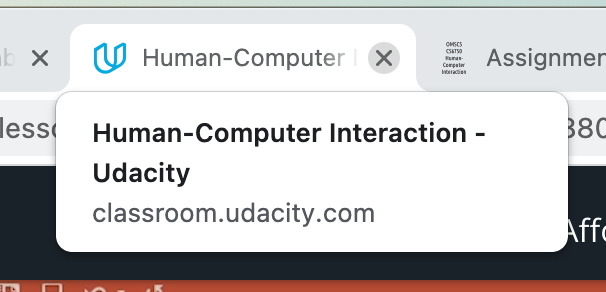
\includegraphics[height=4cm]{jdf-latex/Figures/close a tab.png}
	\caption{Close a tab in Chrome}
	\label{fig:closeatab}
\end{figure}

\subsubsection{Mapping}
\begin{quotation}
\noindent “Mapping is a technical term ... meaning the relationship between the elements of two sets of things."
- Don Norman
\end{quotation}

The mapping is a great principle to offload the user's cognitive effort. It can help to mitigate the gulfs of execution, especially in what action to take and how to execute in the interface. Also, it can help to feedback intuitively that bridge the interpretation and evaluation of gulfs of evaluation. For example, when you want to add an event in the calendar app, it is easy to understand you should click the time slot you would like to add an event. And once finished, you can easily evaluate since the calendar interface will show that event in the expected time slow. The user experience is mapped between a calendar app and the actual calendar. That helps to bridge both gulfs of execution and gulfs of evaluation.

\begin{figure}[h]
	\centering
	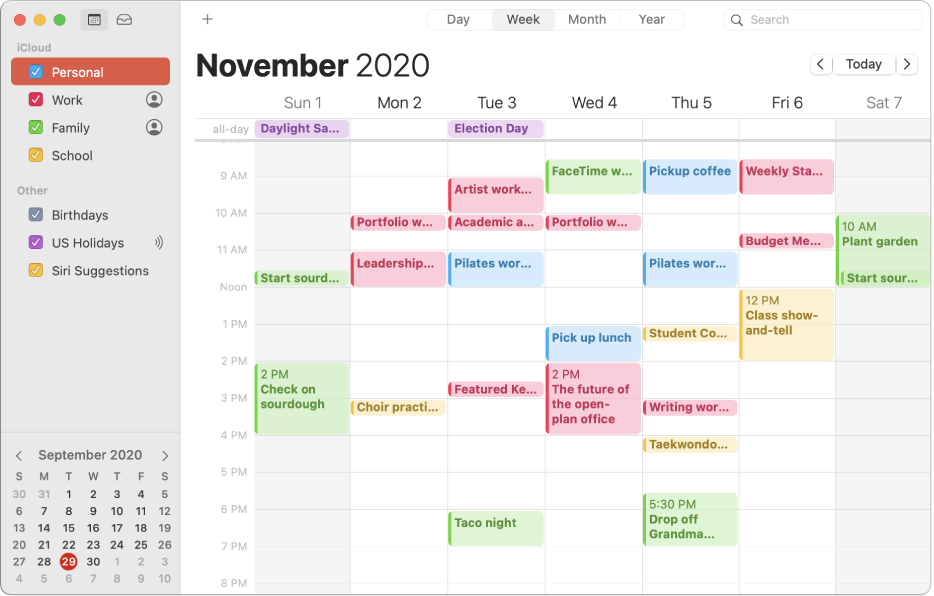
\includegraphics[height=6cm]{jdf-latex/Figures/calendar.png}
	\caption{Calendar App}
	\label{fig:calendar}
\end{figure}

\subsubsection{Consistency}
\begin{quotation}
\noindent “Consistency in design is virtuous. It means that lessons learned with one system transfer readily to others. ... If a new way of doing things is only slightly better than the old, it is better to be consistent."
- Don Norman
\end{quotation}

Consistency helps to bridge the gulfs of execution, especially on identifying actions and executing in interfaces. For example, in most of the system keyboard shortcut "CMD + W" means close the current window. So in the Chrome app, using "CMD + W" is also closing the current tab. Almost in all Mac applications, doing "CMD + W" will close the current window. This help to bridge the gulfs of execution that users do not have to learn which actions to take or how to execute to close a window. It is always the same set of commands.

\subsection{Principles to create interfaces that emphasize the participant view}
The two principles that can be used to create interfaces that emphasize the participant view of the user are Equity and Tolerance.

\subsubsection{Equity}
\begin{quotation}
\noindent “The design accommodates a wide range of individual preferences and abilities."
- Ronald Mace
\end{quotation}

Equity helps to create an interface suitable for a different context. For example, on the web page, there is often a button to choose multi-languages. It cares about not only the user's abilities but also the language background. Also, the latest smartphones can let you adjust the brightness with your preference. So different people can use the interface in their desired brightness. The equity principle helps to consider the context when designing the interface.

\subsubsection{Tolerance}
\begin{quotation}
\noindent “Users often choose system functions by mistake and will need a clearly marked 'emergency exit' to leave the unwanted state without having to go through an extended dialogue. Support undo and redo."
- Don Norman
\end{quotation}

Tolerance is important for the interface to consider the context. For example, it is easy to make typos when one is typing. The writing interface should be able to take care of the context when the user is typing wrongly and allow the user to undo it. By designing an interface allowing the user to make mistake, the tolerance principle helps to create interfaces that emphasize the participant view.

\section{Q2 - Principles to help payment checkout page}
\subsection{Interface that is intolerant of errors}
We do much more online shopping since COVID. One of the interfaces that are intolerant of errors the user commits is the checkout page. It is by nature that you have to key in all the information correctly, otherwise, the transaction will not go through. To make the transaction, one need to key in all card numbers, names, expired dates, secure code correctly within a given time limit. Since it is a 16 digits code with other numerical information, it can easily go wrong especially for the elderly. One digit wrong, normally you have to start over and key in all the information again. The transaction will only happen when you have all the numbers and information correct.

\begin{figure}[h]
	\centering
	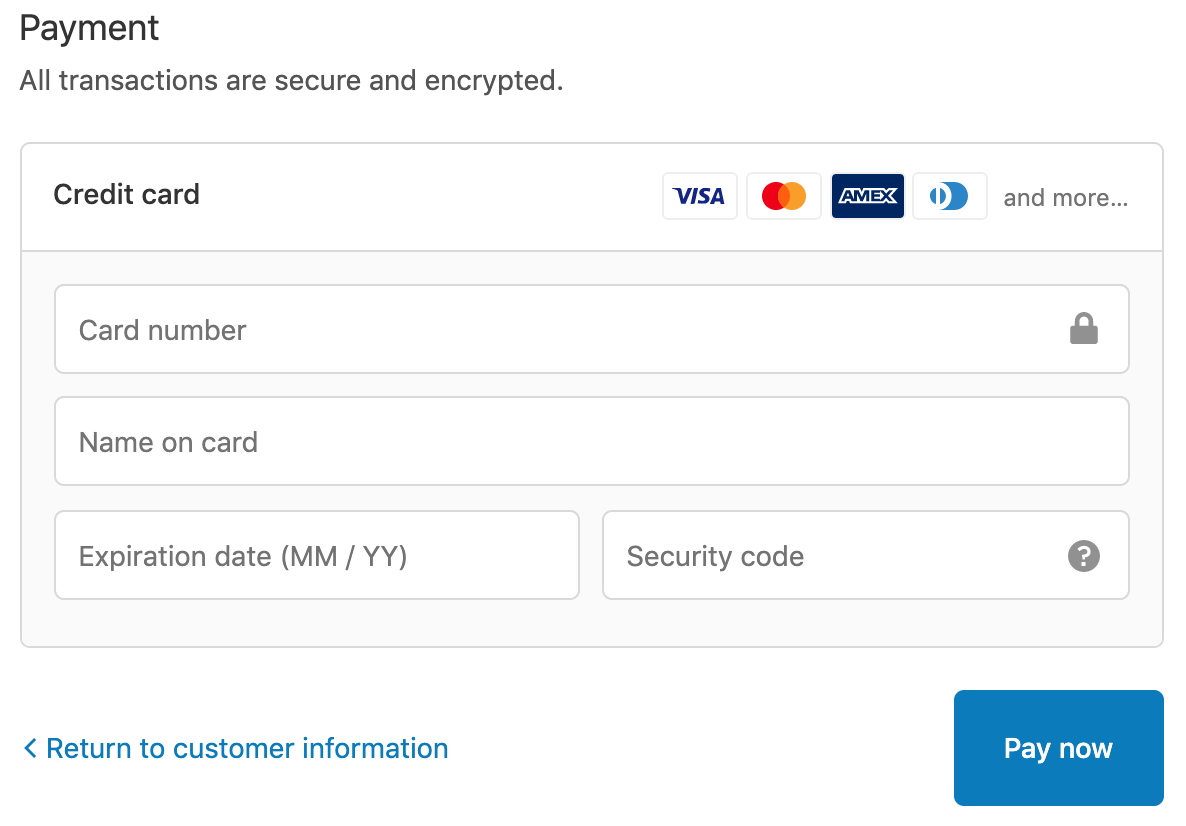
\includegraphics[height=6cm]{jdf-latex/Figures/shopify_onsite.png}
	\caption{Checkout payment page}
	\label{fig:shopify_onsite}
\end{figure}

\subsection{Constraints, improved mappings and improved affordances}
\subsubsection{Constraints}
We can have the interface only allow numbers in the number box, thus will reduce the chance that people key in dashes or spaces in the card number box. Also, we can have 4 boxes with each allow only 4 digits, to further avoid the chances people key in less or more numbers.

\subsubsection{Improved Mappings}
The interface can have a layout that looks like a credit card. That will map the user's experience of using a credit card. People will know what information to look for on their credit card. It will bridge the gulfs of execution in this case.

\subsubsection{Improved Affordances}
The interface can use a signifier to help with perceived affordance. For example, a pop up to indicate what is a secure code, or what is the expired date. It will help to bridge the gulfs of execution as well and make it easier for the user to understand what information to fill in.

\section{Q3 - Game with slips and mistakes}
The game that easy to make slips or mistakes is FIFA. It is a challenging video game and people tend to make a lot of slips or mistakes in the beginning and gradually learn how to work with the Xbox controller.

\begin{figure}[h]
	\centering
	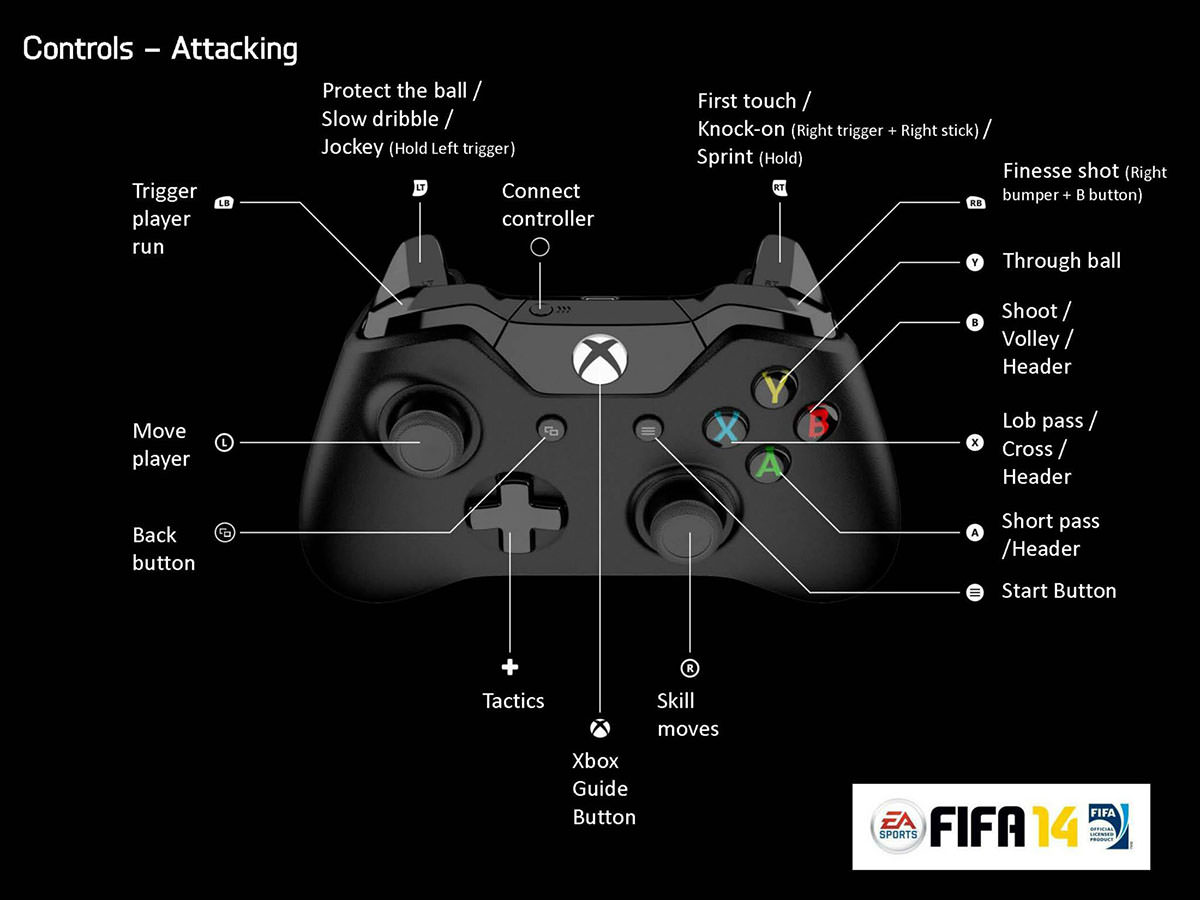
\includegraphics[height=6cm]{jdf-latex/Figures/xbox.jpeg}
	\caption{FIFA Xbox controller}
	\label{fig:xbox}
\end{figure}

\subsection{Slips in game}
People tend to make slips in FIFA even for the expert player. After learning the interface for a while, people understand which buttons on the interface are mapped to which actions of the player on screen. But we can still make a mistake that instead of pressing B for shooting, we accidentally press X for crossing. It is a common slip people will make especially when they just start to play FIFA. It happens because there is no mapping between the buttons and the actions player will take. Through practice, people can gradually map the B button to shooting action. But it requires cognitive effort and people may forget it from time to time and make a slip.

The interface can help to prevent that slip by adding a controller on the foot. It uses the mapping principle to help people to remember which action to take when he wants to perform a shooting action.

\subsection{Mistakes in the game}
Generally, novice users tend to make mistakes in the game. For example, many advanced actions need users to press multiple buttons to perform. Auto defence needs the player to hold 2 buttons together, and LB and joystick need to be press together to perform acceleration. People tend to make the mistake that they do not know what to do when they want to do certain actions. It is caused by the complex interface and it is challenging for the user to remember all the button to action mappings.

The interface can have many tutorials with instructions for the user to remember how to do certain actions. To incentive the user to learn, the interface can reward the player to go through the tutorials.

\subsection{Challenges in the game}
It is challenging to score in the FIFA game. There is a goalkeeper to stop most of the users' attempts. It is by design to make the game challenging and the users have to learn how to shoot with the best power and angle. 

\section{Q4 - Good and bad representations in interfaces}
Good representations: (Joyner, 2021c)
\begin{enumerate}
	\item Make relationships explicit.
	\item Bring objects and relationships together.
	\item Excludes extraneous details.
	\item Expose natural constraints.
\end{enumerate}


\subsection{Good representation interface}
\subsubsection{Connections between the representation and the underlying content}
One interface that is using good representation is the calculator app of Mac. The interface mimics the actual calculator, so the representation of the interface is directly mapped to the underlying content. The user has no cognitive effort to understand how to use it if he has used an actual calculator before. 

\begin{figure}[h]
	\centering
	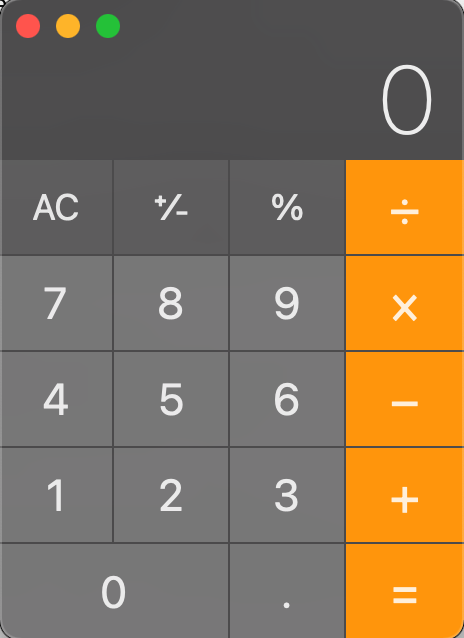
\includegraphics[height=4cm]{jdf-latex/Figures/calculator.png}
	\caption{Mac Calculator}
	\label{fig:calculator}
\end{figure}

\subsubsection{How does the interface exemplify two criteria of a good representation}

The calculator interface makes the relationship explicit. It looks like the interface of a real calculator. So it is easy for the user to understand what each button is used for. It matches the mental model exactly and offloads most of the cognitive load.

The calculator interface also excludes extraneous details. It shows the basic interface, and one can switch to the scientific calculator if needed. It does not have an on/off button like the real calculator since it is not relevant to the calculation task.

\subsection{Bad representation interface}
One interface that is using bad representation is the command line interface. I often need to google to understand what actions to take for the task I want to complete.
\begin{figure}[h]
	\centering
	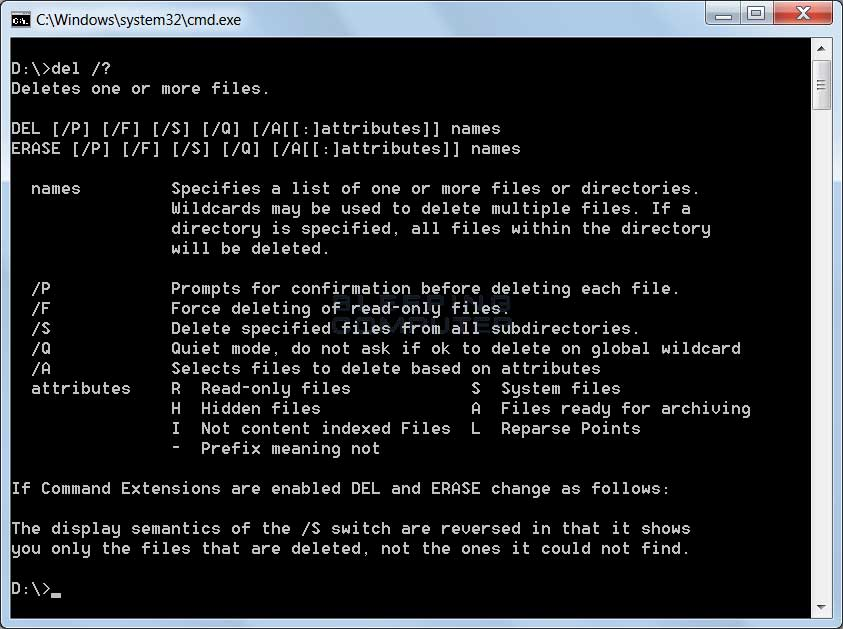
\includegraphics[height=5cm]{jdf-latex/Figures/commandline.jpeg}
	\caption{Command Line Interface with poor representation}
	\label{fig:commandline}
\end{figure}
\subsubsection{Mismatches between the representation and the underlying content}

There are no direct relationships between tasks and the commands in the command line. For example, to move a file to another folder, rather than drag in the UI, you have to type "mv path/to/file path/to/destination". If one replaces command "mv" to "move", the task will fail. It is not intuitive and takes much cognitive effort to remember all the commands for the tasks. And the actions to take can be difficult to remember, such as "git checkout -b test <name of remote>/test" to copy a remote branch to local for the version control purpose. There is no way to map the representation with the underlying content.

\subsubsection{How does the interface violate two criteria of a good representation}
The representation of this interface does not bring the objects and relationships together. It is hard to understand how to perform certain tasks. There is a slow learning curve for using the command-line interface to complete certain tasks. 

The command-line interface also violates the criteria that make the relationship explicit. There is no explicit relationship between the commands and actions. There are documentations and manuals, but the combination of commands are endless and you can complete certain tasks using multiple ways. It further increases the difficulty to be proficient in this interface.

\section{References}
[1] Joyner, D. (2021a). Gulf of Execution. Udacity.

https://classroom.udacity.com/courses/ud400/lessons/9129419879/

concepts/91335799740923

[2] Joyner, D. (2021b). Gulf of Evaluation. Udacity.

https://classroom.udacity.com/courses/ud400/lessons/9129419879/

concepts/91335799770923

[3] Joyner, D. (2021c). Characteristics of Good Representations. Udacity.

https://classroom.udacity.com/courses/ud400/lessons/9430399198/

concepts/94375211040923


\end{document}